% Grayscale PATRM engine inside the Zynq-7000 (step 2.2).
% Black and white, no fills. Dashed border = new or changed versus the paper [1].
% Compile: pdflatex patrm_gray_top.tex
\documentclass[varwidth=true, border=6pt]{standalone}
\usepackage[T1]{fontenc}
\usepackage{lmodern}
\usepackage{caption}
\usepackage{tikz}
\usetikzlibrary{arrows.meta, positioning, fit, calc}

\tikzset{
  mod/.style    = {draw, thick, align=center, font=\small, minimum height=11mm, minimum width=24mm, inner sep=2pt},
  newmod/.style = {mod, dashed},
  ps/.style     = {draw, thick, align=center, font=\small, minimum height=10mm, minimum width=26mm},
  port/.style   = {draw, thin, align=center, font=\scriptsize, minimum height=5mm, minimum width=18mm},
  region/.style = {draw, thick, rounded corners=3pt, inner sep=7pt},
  data/.style   = {-{Stealth[length=2.2mm]}, thick},
  ctl/.style    = {-{Stealth[length=2mm]}, thin},
  lbl/.style    = {font=\scriptsize, align=center, fill=none},
}

\begin{document}
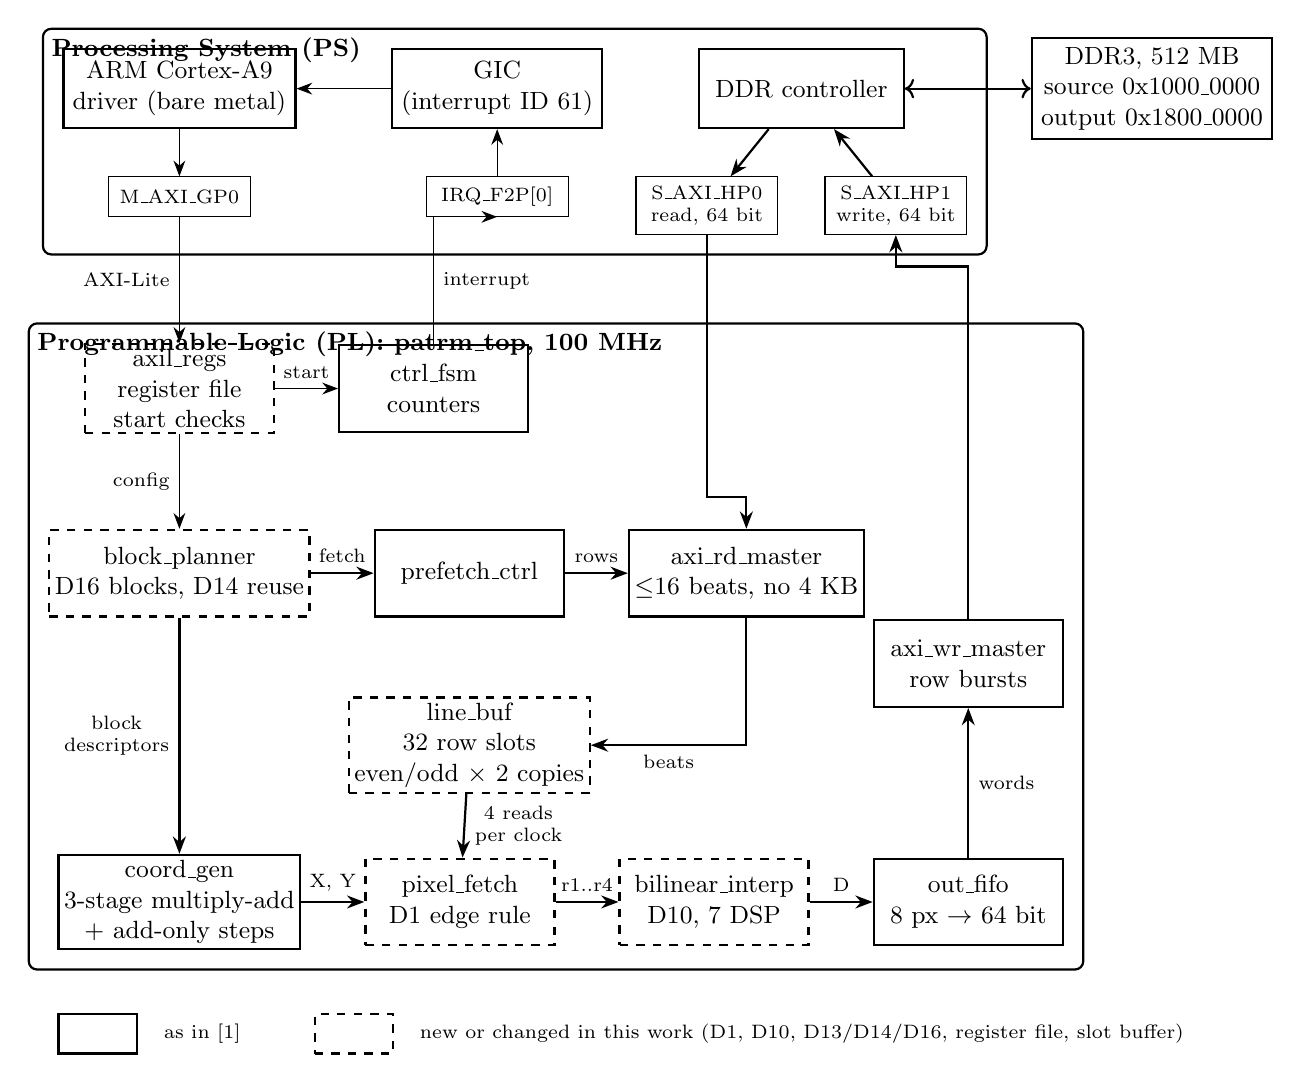
\begin{tikzpicture}[node distance=7mm and 8mm]

% ---------------- Processing system ----------------
\node[ps] (arm) at (0,0) {ARM Cortex-A9\\driver (bare metal)};
\node[ps, right=12mm of arm] (gic) {GIC\\(interrupt ID 61)};
\node[ps, right=12mm of gic] (ddrc) {DDR controller};
\node[port, below=6mm of arm] (gp0) {M\_AXI\_GP0};
\node[port, below=6mm of gic] (irq) {IRQ\_F2P[0]};
\node[port, below=6mm of ddrc, xshift=-12mm] (hp0) {S\_AXI\_HP0\\read, 64 bit};
\node[port, below=6mm of ddrc, xshift=12mm] (hp1) {S\_AXI\_HP1\\write, 64 bit};
\node[region, fit=(arm)(gic)(ddrc)(gp0)(irq)(hp0)(hp1),
      label={[font=\small\bfseries, anchor=north west]north west:{Processing System (PS)}}] (psbox) {};
\draw[ctl] (arm) -- (gp0);
\draw[ctl] (irq) -- (gic);
\draw[ctl] (gic) -- (arm);
\draw[data] (ddrc) -- (hp0);
\draw[data] (hp1) -- (ddrc);

% ---------------- DDR ----------------
\node[ps, right=16mm of ddrc, minimum width=30mm] (ddr) {DDR3, 512 MB\\source 0x1000\_0000\\output 0x1800\_0000};
\draw[data, <->] (ddr) -- (ddrc);

% ---------------- Programmable logic: engine ----------------
% control row
\node[newmod, below=16mm of gp0] (regs) {axil\_regs\\register file\\start checks};
\node[mod, right=of regs] (fsm) {ctrl\_fsm\\counters};

% read path row
\node[newmod, below=12mm of regs] (plan) {block\_planner\\D16 blocks, D14 reuse};
\node[mod, right=of plan] (pref) {prefetch\_ctrl};
\node[mod, right=of pref] (rdm) {axi\_rd\_master\\$\le$16 beats, no 4 KB};
\node[newmod, below=10mm of pref] (lbuf) {line\_buf\\32 row slots\\even/odd $\times$ 2 copies};

% pixel path row
\node[mod, below=10mm of plan, yshift=-20mm] (cg) {coord\_gen\\3-stage multiply-add\\+ add-only steps};
\node[newmod, right=of cg] (pf) {pixel\_fetch\\D1 edge rule};
\node[newmod, right=of pf] (ip) {bilinear\_interp\\D10, 7 DSP};
\node[mod, right=of ip] (of) {out\_fifo\\8 px $\to$ 64 bit};
\node[mod, above=of of, yshift=12mm] (wrm) {axi\_wr\_master\\row bursts};

\node[region, fit=(regs)(fsm)(plan)(pref)(rdm)(lbuf)(cg)(pf)(ip)(of)(wrm),
      label={[font=\small\bfseries, anchor=north west]north west:{Programmable Logic (PL): patrm\_top, 100 MHz}}] (plbox) {};

% ---------------- connections ----------------
\draw[ctl] (gp0) -- node[lbl, left] {AXI-Lite} (regs);
\draw[ctl] (regs) -- node[lbl, above] {start} (fsm);
\draw[ctl] (fsm.north) |- node[lbl, pos=0.25, right] {interrupt} (irq.south);
\draw[ctl] (regs) -- node[lbl, left] {config} (plan);

\draw[data] (plan) -- node[lbl, above] {fetch} (pref);
\draw[data] (pref) -- node[lbl, above] {rows} (rdm);
\draw[data] (hp0.south) |- ($(rdm.north)+(0,4mm)$) -- (rdm.north);
\draw[data] (rdm.south) |- node[lbl, pos=0.75, below] {beats} (lbuf.east);
\draw[data] (plan) -- node[lbl, left] {block\\descriptors} (cg);
\draw[data] (cg) -- node[lbl, above] {X, Y} (pf);
\draw[data] (lbuf) -- node[lbl, right] {4 reads\\per clock} (pf);
\draw[data] (pf) -- node[lbl, above] {r1..r4} (ip);
\draw[data] (ip) -- node[lbl, above] {D} (of);
\draw[data] (of) -- node[lbl, right] {words} (wrm);
\draw[data] (wrm.north) |- ($(hp1.south)+(0,-4mm)$) -- (hp1.south);

% ---------------- legend ----------------
\node[mod, minimum width=10mm, minimum height=5mm, below=8mm of cg.south west, anchor=north west] (l1) {};
\node[right=2mm of l1, font=\scriptsize, align=left] (l1t) {as in [1]};
\node[newmod, minimum width=10mm, minimum height=5mm, right=8mm of l1t] (l2) {};
\node[right=2mm of l2, font=\scriptsize, align=left] {new or changed in this work (D1, D10, D13/D14/D16, register file, slot buffer)};

\end{tikzpicture}

\captionof{figure}{Grayscale PATRM engine on the Zynq-7000 (ZedBoard). The ARM programs the register file over
GP0, the engine reads the source over HP0 and writes the output over HP1 (both DDR), and signals the end of a
frame with an interrupt. Based on [1], Fig.~4.}
\end{document}
